\chapter{Background}
\label{cha:Background}

\section{Problem Context}
% Goal of the project? Why am I concentrating on PEP's Trustwords?
The project aims to asses the security of \pep's fingerprint representation "Trustwords". Trustwords aim to sacrifice security for increased usability. The encoding scheme has been designed to assist this by having  the user compare a reduced set of words by about half in comparison to other schemes. To achieve this a larger number of bits are required per word. In this case Trustwords maps 16bits per word providing 65537 different combinations. This is, however, the largest number of bits per words (As show in the Literature Review in Chapter \ref{cha:LiteratureReview}) and pushes the boundaries of a language's usable vocabulary.

This abnormal design choice has not received a security assessment to back up claims. This paper, therefore, aims to rectify this research gap.

However, in order to fully understand the project goal it is important to understand public-key cryptography, the role and functioning of \pep and the role fingerprint comparison has in preventing Man-in-the-middle attacks.

\textbf{TODO:} Maybe research questions here instead of in the literature review

\section{Public-key Cryptography Key Exchange}
Asymmetric cryptography facilitates the secure encryption of messages in end-to-end encryption (E2EE), verification of digital signatures and sharing of pre-communication secrets, among others. The use-case of E2EE messages will be the primary focus of this paper.

The asymmetry stems from the use of "Public" and "Private" keys. The Public key is used to encrypt data that only the respective Private key can decrypt. This means the keys required to communicate can be easily shared across insecure channels.

To construct an E2EE connection the initial stage will be a key exchange using the key types discussed previously. This is the sharing of a pre-shared secret between two verified parties, this will then be used to encrypt subsequent messages with symmetric encryption\footnote{This is due to the speed increase of symmetrical over asymmetrical encryption}. This, however, hinges on the verification of the initial parties, if one party impersonates another and gets to view the pre-shared secret all communication becomes decryptable. Therefore, the correct identification of parties is crucial to maintaining secure communication channels. The exploitation of this is known as a Man-in-the-middle (MiTM) attack. This can be bidirectional where the attacker can sit in the middle of a communication channel and decrypt all correspondence. Figure \ref{fig:mitm} contains a visual representation of this attack.

\begin{center}
    \newcommand{\tgap}{0.1cm}

\begin{center}
\begin{tikzpicture}[
	every node/.style={fill=white},
    diagram item/.style={},
    align=left
]         

\node (Router)[
    diagram item,
    label=above:Alice,
    yshift=-2cm
] {
\includegraphics[scale=\ciscoImageScale]{\cisco/workstation}};

\node (Victim)[
	diagram item,
	label=above:Bob,
	right of=Router,
	xshift=7cm
] {
\includegraphics[scale=\ciscoImageScale]{\cisco/workstation}};

\coordinate (CENTER) at ($(Victim)!0.5!(Router)$);
\node (Attacker)[
	label=below:Eve,
	below of=CENTER,
	yshift=-3.5cm
] {
\includegraphics[scale=\ciscoImageScale]{\cisco/laptop}};

\draw[-] (Router)--node[yshift=0.5cm]{Old Connection}(Victim);
\draw[red, very thick] (Router)--node{New Connection}(Attacker);
\draw[red, very thick] (Attacker)--node{New Connection}(Victim);


\end{tikzpicture} 
\end{center}

    \begin{figure}[h]
        \caption{Photo depicting a MITM attack}
        \label{fig:mitm}
    \end{figure}
\end{center}

Due to the assumption that the attacking party (Eve) does not have the same public-private key pair as either party (Alice or Bob) the fingerprint of the public key can be used for identification. There are, however, issues in how a user should link a key's fingerprint to real world entity. This paper will, however, assume that users know the respective parties' correct fingerprint, as the protocols used to achieve this are outside the project's scope.

The fingerprint of the key is generated by running the main components of the key through a secure one way hash function\footnote{Explain this?}. This process produces a digest of fixed length that can be used to compare keys. Therefore, the comparison of expected and actual fingerprints is used to detect MiTM attacks and prevent impersonation.

\section{PGP}
Pretty Good Privacy (PGP) is a specific implementation of public key cryptography discussed in the previous section. Its main use-case is for securing message based communications but can also be used for file or hard drive encryption.

Each element of a PGP key is split into what is know as a 'packet'. The 'fingerprint' packet v4 contains a version number, timestamp and the main elements of the keys algorithm (i.e. RSA exponent and modulus) formatted as MPIs\footnote{Multiprecision integers are unsigned integers used to hold large integers such as the ones used in cryptographic calculations.}. This data is then preceded with PGP packet header (used to specify length and version numbers). This is all then utilized as input into the one-way hash function SHA-1 to produce a 160-bit digest.

\textbf{TODO: } Generate an image of PGP v4 fingerprint packet

\newpage

\section{Pretty Easy Privacy}
\begin{wrapfigure}{r}{5cm}
    \centering
    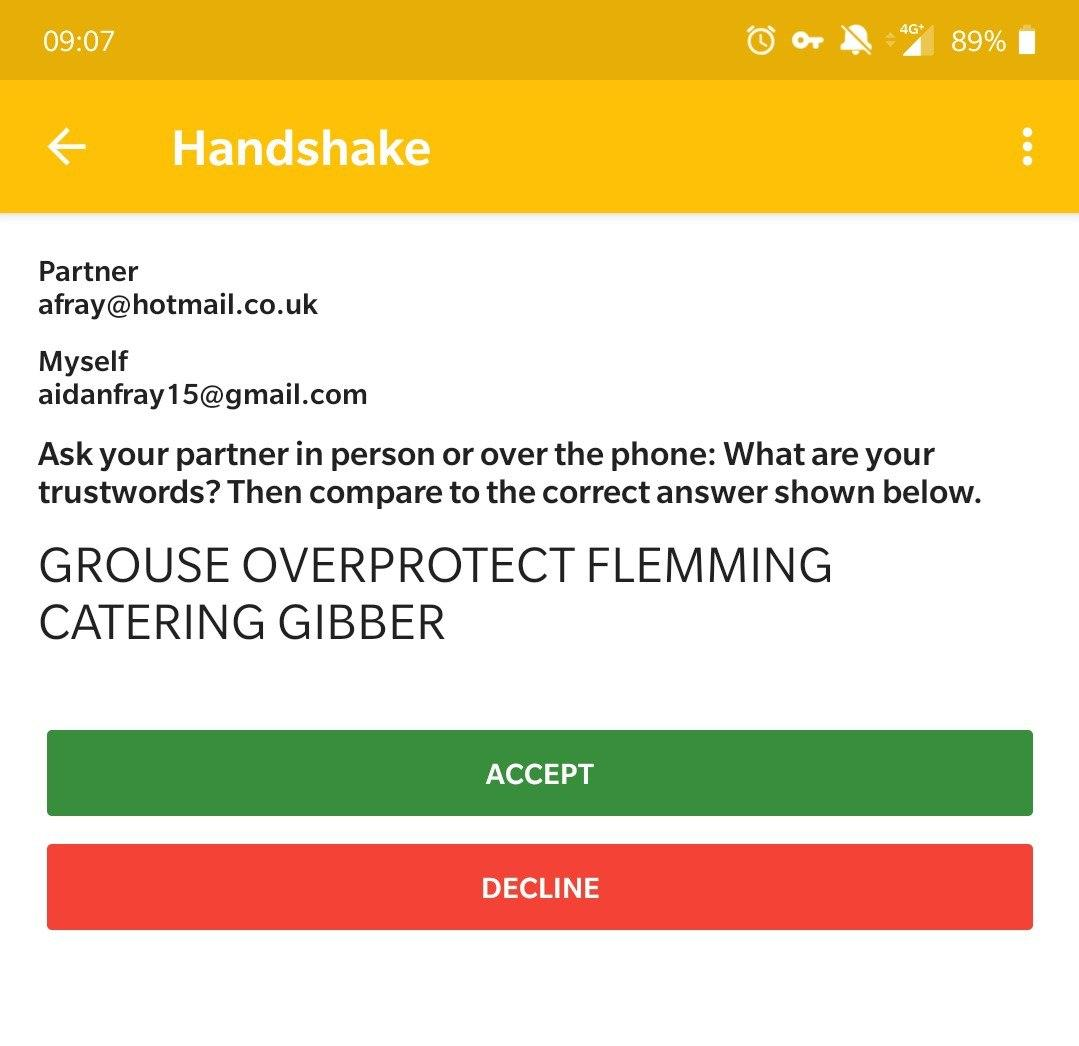
\includegraphics[scale=0.15]{trustwords/trustword_handshake.jpg}
    \caption{Trustword fingerprint verification}
    \label{fig:trustwords}
\end{wrapfigure}

Pretty Easy Privacy (\pep) is a data encryption system that utilises PGP encryption to provide E2EE on all common channels of communication such as email of SMS. \pep's design principles state that above all the systems should be easy to install, use and understand.

\pep deals with the threat of MiTM attacks by having users compare the respective key fingerprints encoded as a set of words. Figure \ref{fig:trustwords} shows the \pep Android implementation of trustwords. The user pair of users then authenticate the words on an OOB (Out of Band) channel such as a phone call or in-person communication. If both users decide the words match they will accept or decline respectively.

The trustwords are unique for each pair of keys, this is the alternative of having a static key for each user. The justification behind the unique set for each user pair is in an attempt to motivate users to perform the authentication ceremony. The unique combined fingerprint is believed to reduced complacency due to inherent change \textbf{[CITE ME]}. 

Each key pair is the exclusive-or of each key's fingerprint, this combined values is then broken down into 16-bit chunks and mapped to words via a pre-defined dictionary.

\begin{figure}[h!]
    \centering
    $KeyFingerprint_{1} \oplus KeyFingerprint_{2} = TrustwordsFingerprint$
    \caption{Creation of the combined Trustword fingerprint}
\end{figure}

\begin{wrapfigure}{r}{5cm}
    \centering
    \begin{BVerbatim}
    [...]
52127 ZYGOTE
52128 ZYGOTIC
52129 ZYMURGY
52130 AACHEN
52131 AARDVARK
52132 AAREN
    [...]
    \end{BVerbatim}
    \caption{Re-mapping position in Trustword dictionary}
    \label{fig:remap}
\end{wrapfigure}

Due to the number of words required ($2^{16}$) alongside the design choice to exclude slang and profanities the english Trustword dictionary requires dual-mapping of a section of words. Approximately 13633/65536 (20.8\%) of words are re-mapped in the dictionary leaving 51903 unique words. The re-mapping is also done on a loop with it remaining alphabetical. Figure \ref{fig:remap} shows the position in the dictionary where this occurs. This predictability within the dictionary will be explored later in the paper.




% Does this need explaining?
\section{OpenCL}

\section{Similarity metrics (Soundex etc)}